\chapter{Introduction}
\label{ch:intro}
Unmanned Aerial Vehicles (UAV), more familiarly known as drones, are
increasingly of great use in applications such as aerial
surveillance\cite{dronesurvey1, dronesurvey3}, transporting
medicines\cite{dronedelivery1,dronedelivery2}, photography\cite{dronephoto1,
dronephoto2, dronephoto3}, archeology\cite{dronearchaeology}.
Due to their ability to go to inaccessible areas e.g., terraces of high rise
buildings, hills, etc., it is indispensable in search and rescue operations.
Drones have reportedly been used in search and rescue operation in flood hit
areas in Uttarakhand in 2013. These have also been used for military
purposes e.g., surveillance to restrict infiltration in border areas\cite{dronesurvey2}.
Areas such as agriculture(for pest control), public health (stacked garbage
detection), civil inspection (dams, nuclear reactors, old temple restoration) have 
opened a lot of opportunities towards utility of drones.

Drones may be classified in two types: those which can hover (e.g.
quadcopters, octopcopters, etc.), those which cannot (mainly military drones
used for surveillance, attack etc.). We are mainly interested in the first type due
to ability to capture still photographs and videos. It enables us to do
close inspection which is required in many applications. Currently, in the
market variety of quadcopters are available from USD 100 to USD 3000.
Some of the models are shown in Figure~\ref{fig:quadcopters}.
Each one has its own specialty. However, for autonomous navigation we require mainly
three characteristics. First, it should have camera with good resolution (at
least 1080 x 720 pixels). Second, it should be able to communicate with a
computer through some protocol and third, we should be able to fly it indoors as
well as outdoors.

\begin{figure}[h!]
\centering
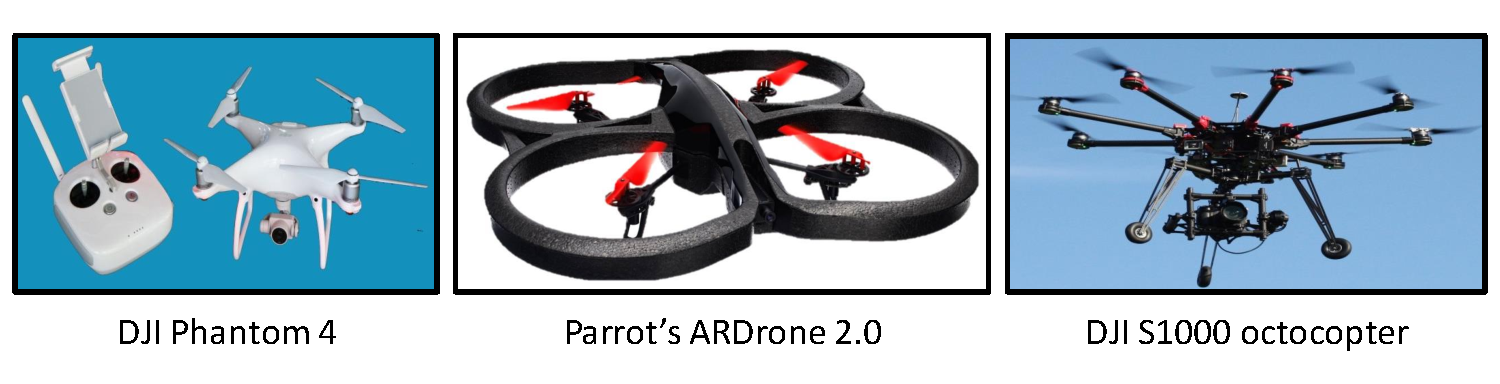
\includegraphics[width=0.98\linewidth]{figures/quadcopters}
\caption[Different models of quadcopters]{Different models of
quadcopters.[Picture Courtesy: Google image search]}
\label{fig:quadcopters}
\end{figure}

Generally the first requirement is met in all quadcopters, but only a few
quadcopters satisfy second and third requirements. E.g., DJI Phantom 4
 has camera mounted on 3-axis gimbal coupled with gyroscope. It enables
us to take very stable video while flying. But, till now there is no way to interface DJI
Phantom 4 with a computer. We have to use joystick like control provided along
with the quadcopter to manually navigate the quadcopter.
Octcopters such as  DJI S1000 have excellent flight control as well as
stability. But due to its bulky nature (weight around 11Kg), we can not use it
in indoor areas.



There are a few assembled quadcopter systems which became quite popular lately,
e.g., team at the University of Pennsylvania have developed a series of
quadcopters capable of doing unbelievable maneuvers. However, such systems use motion camera
systems such as Vicon to find out the pose of the quadcopters in motion.
Hence, we cannot use it in uncontrolled environments.

Parrot's ARDrone and Bebop are two reasonably priced (USD 350 and USD
700 respectively) quadcopters having HD camera with resolution 1280 x 720
pixels. Though it is lightweight (compared to DJI Phantom 4), it is robust
enough to withstand in outdoor conditions. It streams a WiFi hotspot to which
any computer can be connected. Parrot has also released SDK which is helpful to
do interfacing with these quadcopters. As Parrot's Bebop was not publicly
released until the end of 2015, we have used Parrot's ARDrone 2.0.

\section{Motivation}
%There are two main challenges in using drones for various applications.
%One of them is proper navigation and control of the drone, and another is
%the analysis of images captured by the camera to understand the scene.

Consider a case where  we are inspecting a dam for cracks. We need to ensure
that all small cracks are detected along with their respective positions from
the captured video. Manual inspection of videos is prone to (human) errors. 
So we need to develop an efficient algorithm to process the video and output
desirable representation of the input scene. One of the useful representations
is a full panoramic view of the dam constructed from closeups of the patches. 

However, large featureless regions of surfaces like a dam pose challenges to
the use of homography based stitching to create the panorama. Hence, there is a
requirement of a method which can incorporate additional information available from drone to do
mosaicing of scenes with vacant spaces. 

We need to navigate the quadcopter smoothly to image large planar surfaces in
order to get good quality images from closeup. Developed countries like the US
have been using military grade drones with superior technology which enables us to
navigate a drone with point precision. But as these drones are very expensive,
their use is limited in developing countries. Also, as these drones use the GPS
for navigation, we cannot use them in indoor scenes. Even if the GPS signal is
available, we cannot rely only on GPS for navigation of drones due to various
reasons (GPS jamming, spurious GPS signals). We may think of navigating drone
manually in such cases. It will however be cumbersome and prone to human errors.
Hence, there is need of developing a stable technique for autonomous navigation
and control of drones in various scenarios.

Imaging large planar surfaces using single quadcopter in one flight is not
feasible due to battery constraints. In such cases, one may use multiple
quadcopters in collaboration to complete the task. Robust identification of
each quadcopter under motion is needed for using multiple quadcopters. Fiducial
markers are generally used to robustly identify objects in the environment. But,
current fiducials do not get detected under motion blur as they heavily depend on the
detection of geometric patterns such as lines, corners, etc. Hence, there is a
need of developing blur resilient fiducials which can be detected robustly under
a heavy motion blur.

The problem of autonomous navigation of quadcopters to image multiplanar
surfaces with correctly classifying each quadcopter with the help of blur
resilient fiducial, forms the basis of the work presented in this thesis.\\

\section{Problem Statement}
\textit{We would like to autonomously navigate the quadcopter to image
single as well as multiple planar regions and create a mosaic of the 
scene. We would also like to identify quadcopter under motion robustly for
better collaboration among multiple quadcopters.} 

We decompose our problem of mosaicing a multiplanar scene containing
vacant spaces through the autonomous navigation of one or more quadcopters
into following steps:
\begin{enumerate}
  \item Mosaicing a single planar scene containing vacant spaces through
  quadcopter.
  \item Path planning for imaging a planar scene through quadcopter.
  \item Autonomous navigation of quadcopter for imaging a multiplanar scene.
  \item Unroll the scene spread over multiple planes.
  \item Device a mechanism for robust detection of quadcopter under motion. 
\end{enumerate}
Each of these steps is non-trivial and challenging as explained below. In this
thesis, we deal with these steps by leveraging the information available from a quadcopter.  

\section{Challenges}
The challenges which make our problem interesting to solve are as follows. 
\begin{itemize}
  \item \textbf{Imaging scenes orthographically from close range:}
We need to image scenes in such a way that we can capture finer details
(e.g., cracks in structures like a dam, bridge, etc.). One such example is shown
in Figure \ref{fig:orthographicView}. We need to take the photo
orthographically from close-up in order to get the details of the pressure dial
which are missing from the perspective view taken from the long range. The
dimensions of the wall make it impossible to image it orthographically  using
a handheld camera. 

\begin{figure}[h!]
\centering
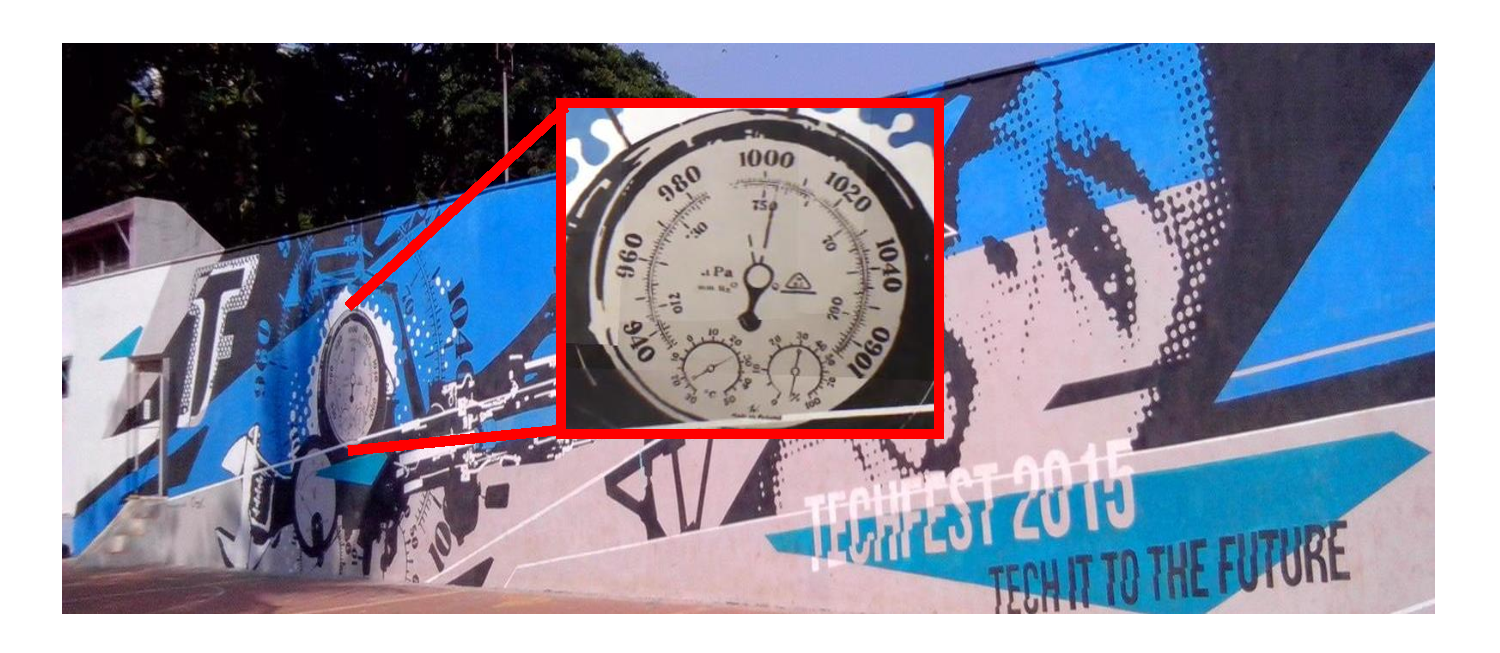
\includegraphics[width=0.98\linewidth]{figures/orthographicView}
\caption[Problems in imaging large scene using handheld camera]{Illustration of
problems in imaging large planar scene with handheld camera. A 40 feet wall
captured with handheld camera from long range doesn't capture smaller details
such as the pressure dial shown in the box. We need to capture such large
planar structures by placing camera closer and orthogonal to the plane being imaged.}
\label{fig:orthographicView}
\end{figure}

\begin{figure}[h!]
\centering
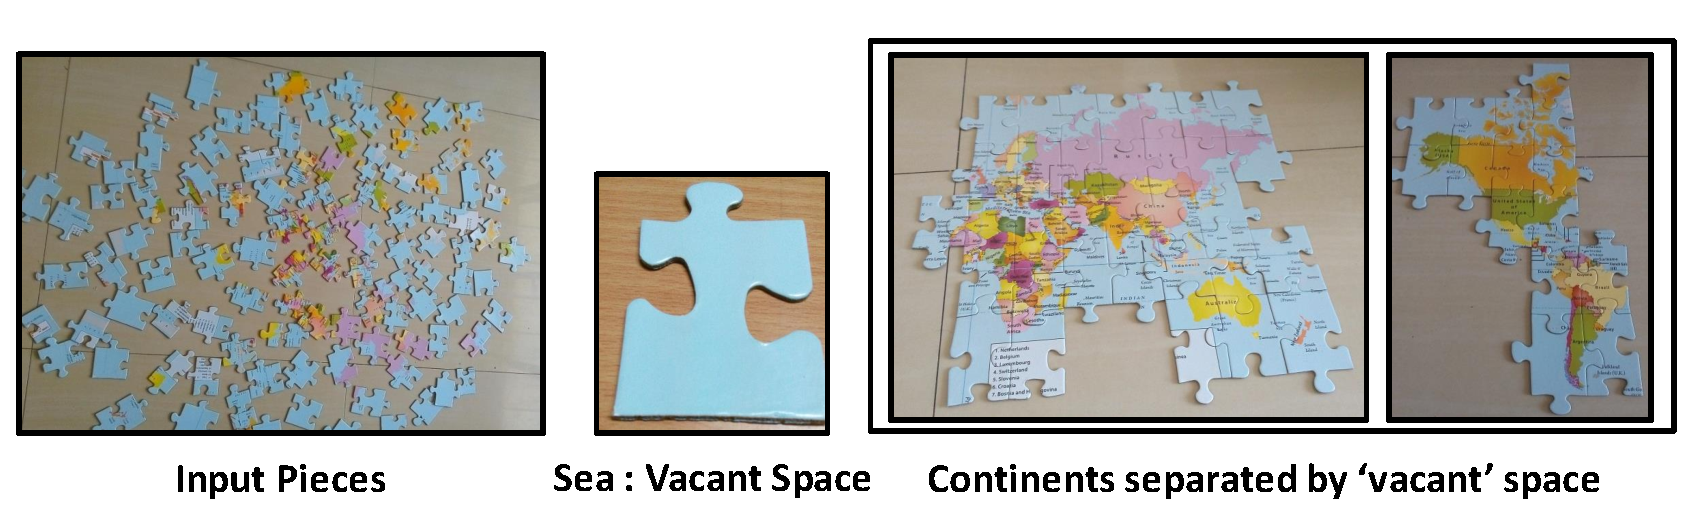
\includegraphics[width=0.98\linewidth]{figures/vacantSpaces}
\caption[Jigsaw Puzzle as a mosaicing problem]{Jigsaw Puzzle as a mosaicing
problem. Individual pieces (Left) of jigsaw puzzle can be thought of constituent images of mosaic. Due to featureless
regions belonging to sea (shown in Middle), one may find it difficult to join
``Americas'' with remaining continents as shown in (Right). We have to use
our knowledge about geography to complete the puzzle.}
\label{fig:vacantSpaces}
\end{figure}
  
  \item \textbf{Vacant spaces and regions with confusing features:} 
  Mosaicing a scene is similar to solving a jigsaw puzzle like one shown in
  Figure~\ref{fig:vacantSpaces}. Blank pieces representing sea make such jigsaw
  puzzle hard to solve because we have to match each and every suitable blank
  piece. We also have to use additional information (e.g., geography in
  the puzzle shown in Figure~\ref{fig:vacantSpaces}) to join different parts
  separated by vacant spaces together.
  
\begin{figure}[h!]
\centering
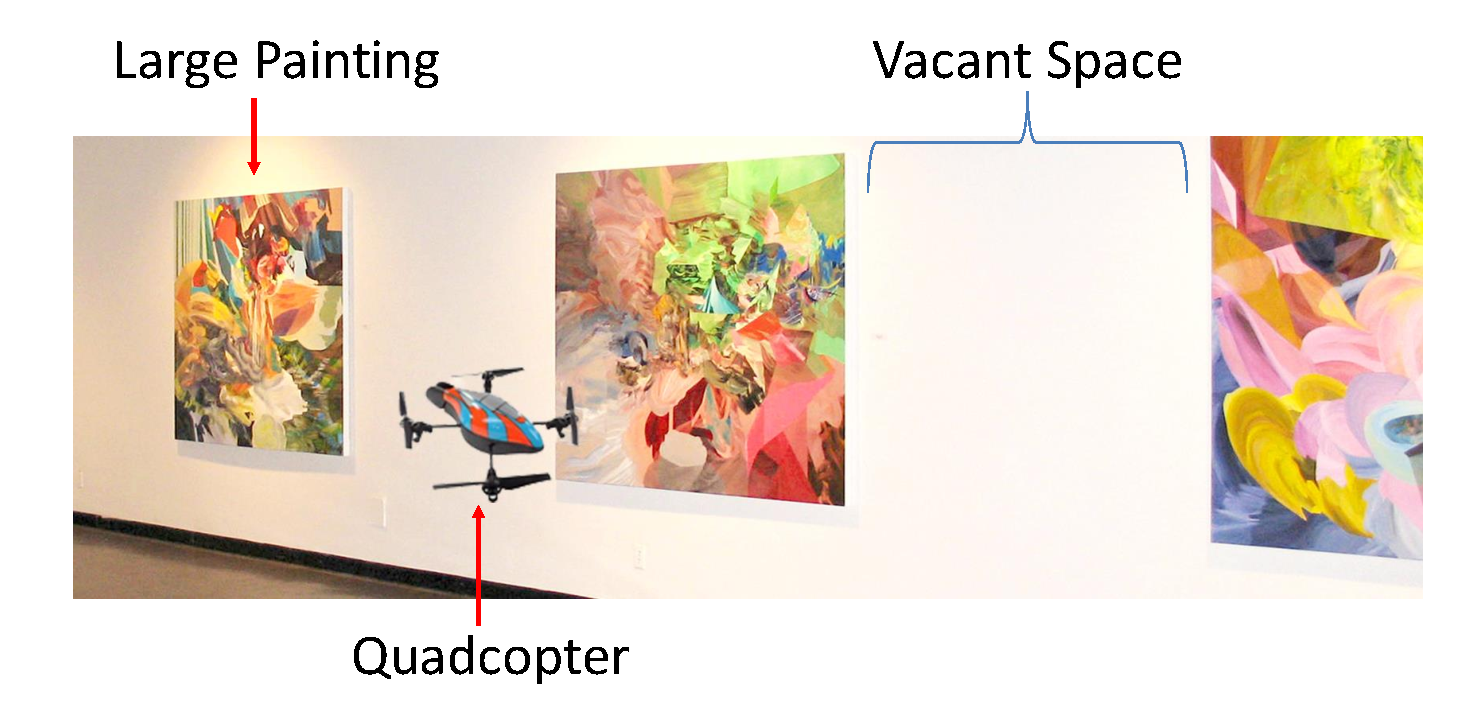
\includegraphics[width=0.98\linewidth]{figures/vacantSpaces/indoor}
\caption[Vacant spaces problem in art gallery]{Vacant spaces are encountered in
various scenes.
When individual portions are captured by a quadcopter, how does one create the complete mosaic
    given that common features are not available as in this example}
\label{fig:indoor}
\end{figure}
  
  Art galleries like the one shown in Figure \ref{fig:indoor}, have exhibits
  separated by empty spaces. If we would like to image these scenes from closeup, we may not
  be able to mosaic the captured images due to vacant space. The standard
  mosaicing method uses feature matching algorithms for estimating homography
  between two images. It requires detection of sufficient features in both
  images. But scenes like Figure~\ref{fig:vacantSpacesExample}(left) contain
  large regions with vacant spaces. Such regions result in very few (or almost
  zero) features which pose a problem for stitching images containing such regions.
  The output (shown in Figure~\ref{fig:vacantSpacesExample}-right) of Adobe
  Photoshop, a popular mosaicing software showcases the inability to
  handle vacant spaces.
  
  \begin{figure}[h!]
\centering
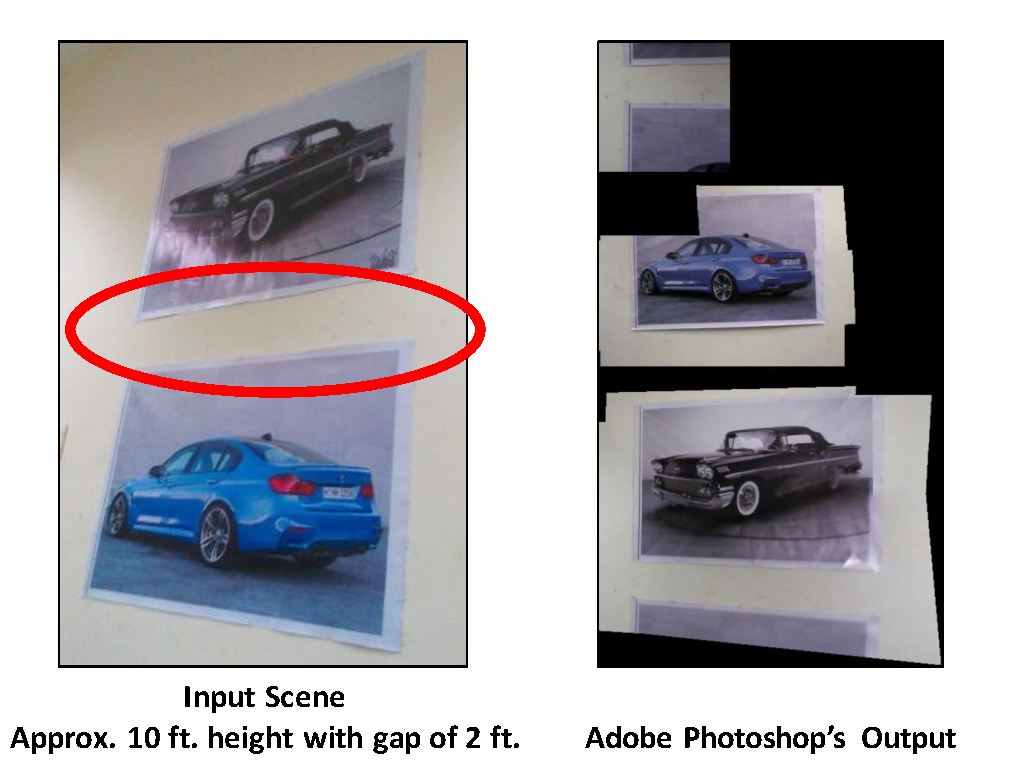
\includegraphics[width=0.98\linewidth]{figures/vacantSpacesExample}
 \caption[Problem of mosaicing scene with vacant spaces using Adobe
 Photoshop]{Is Mosaicing problem solved? Standard stitchers such as Adobe Photoshop can not stitch images which have no or very little features in
 common, such as images with huge vacant spaces.}
\label{fig:vacantSpacesExample}
\end{figure}
 
  Sometimes part of the scene is repeated which confuses the feature matching
  algorithm resulting in images which are not taken from adjacent positions,
  being stitched together (See Figure~\ref{fig:confusingFeatures}).

\begin{figure}[h!]
\centering
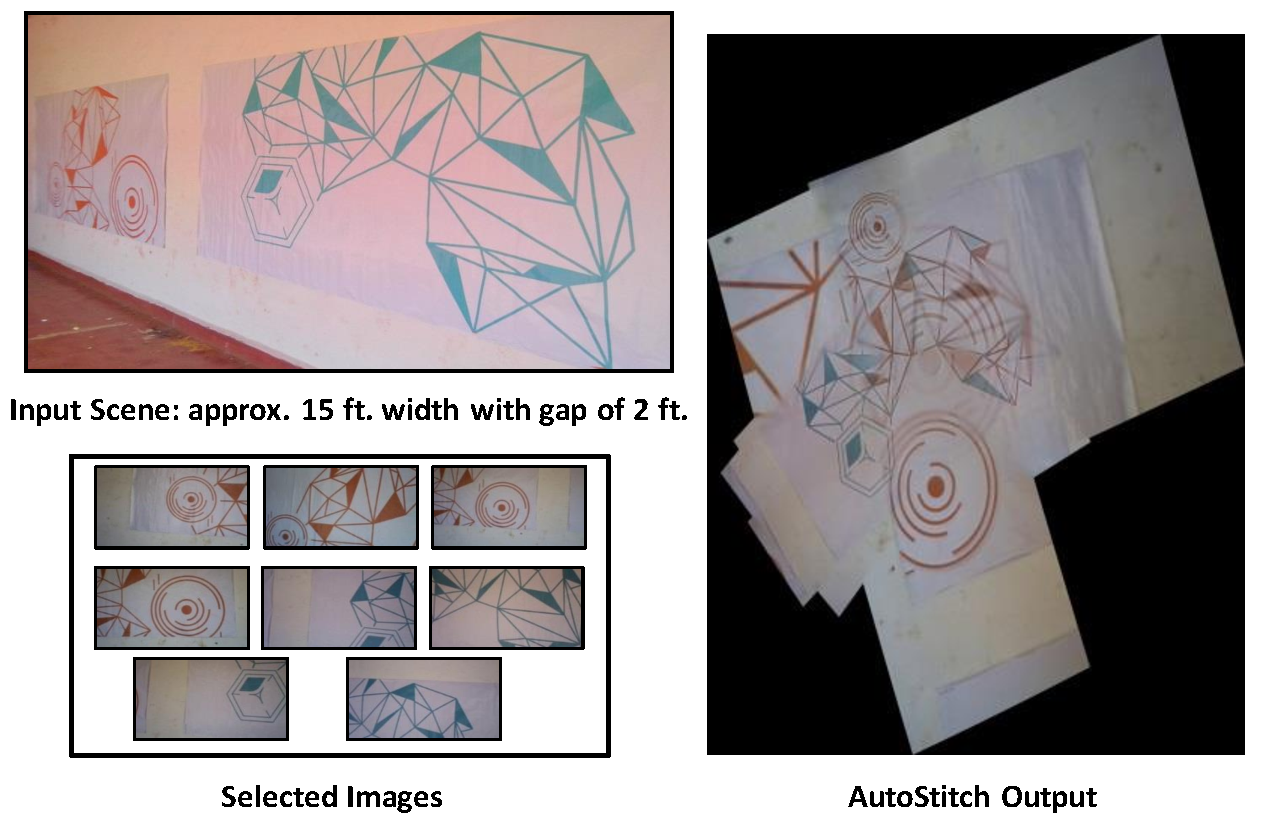
\includegraphics[width=0.98\linewidth]{figures/confusingFeaturesExample}
\caption[Problem of confusing features in AutoStitch]{Repetitive patterns in the
input scene pose a challenge for standard mosaicing methods such as AutoStitch. Images taken from positions
far apart from each other get stitched together as matching algorithm matches
features from those images.}
\label{fig:confusingFeatures}
\end{figure}  

  \item \textbf{Control and navigation of an inexpensive quadcopter:}
  Inexpensive quadcopters like Parrot's ARDrone are very agile and can do
  several maneuvers swiftly. But, controlling it to image large planar regions
  smoothly by keeping a constant distance from the imaging plane is very
  difficult. Also, manual control of quadcopter is a very laborious job. Hence,
  there is need of a mechanism for autonomous navigation of quadcopter to image
  the desired area. Many people use GPS for localizing quadcopter and navigating
  it to the desired location. But GPS based mechanism will not work in indoor areas. 
  Also, we cannot rely on GPS due to various factors such as spurious GPS
  signals, GPS jammers, etc.
  
  \item \textbf{Building a scale accurate 3D map of the environment in
  real-time:} We need accurate 3D coordinates of the region to be imaged on the fly for
  doing efficient path planning. People generally use 3D cameras such as
  Kinect for getting a 3D map of the environment. But, due to payload
  restriction as well as battery requirement, we may not be able to put such
  cameras on top of a quadcopter. The Structure from Motion (SfM) techniques can
  build such a 3D map but due to the real-time requirement, we can not use such
  techniques. Though Engel et al.~\cite{engel} have developed a method to
  create a 3D map for camera based navigation of a quadcopter, it is not precise
  due to inaccuracies in scale. So, we need a
  robust mechanism to build a scale accurate 3D map in real-time.
  
  \item \textbf{Robust Detection of multiplanar bounded regions in real-time:} 
  Multiplanar imaging through quadcopter requires detection of multiplanar
  bounded regions in real-time. There are a few methods like
  multiRANSAC~\cite{zuliani}, j-linkage~\cite{jlinkage},
  t-linkage~\cite{tlinkage} in literature for detection of multiple models from
  the input data.  But, these methods do not output boundaries of planar
  regions. Also, these methods have not considered validity of boundaries of
  planar regions to  filter noisy points appropriately. As a result such noisy
  points get clustered into wrong models, extending boundaries of planar
  regions incorrectly. Hence there is a need of a method to accurately estimate
  multiplanar bounded regions in real-time.
  
  \item \textbf{Identification of a quadcopter under motion:}
  The movement of quadcopters like ARDrone is quite jerky due to its inexpensive
  nature. This results in motion blur in images of quadcopters, which makes
  tracking of quadcopter very challenging. Though we can put fiducials such as
  ARTag on the quadcopter to keep the track, such fiducials are not detected
  due to motion blur. Figure \ref{fig:ARTagBlur}, demonstrates the problem in
  detection of ARTag under motion blur.
  
\begin{figure}[h!]
\centering
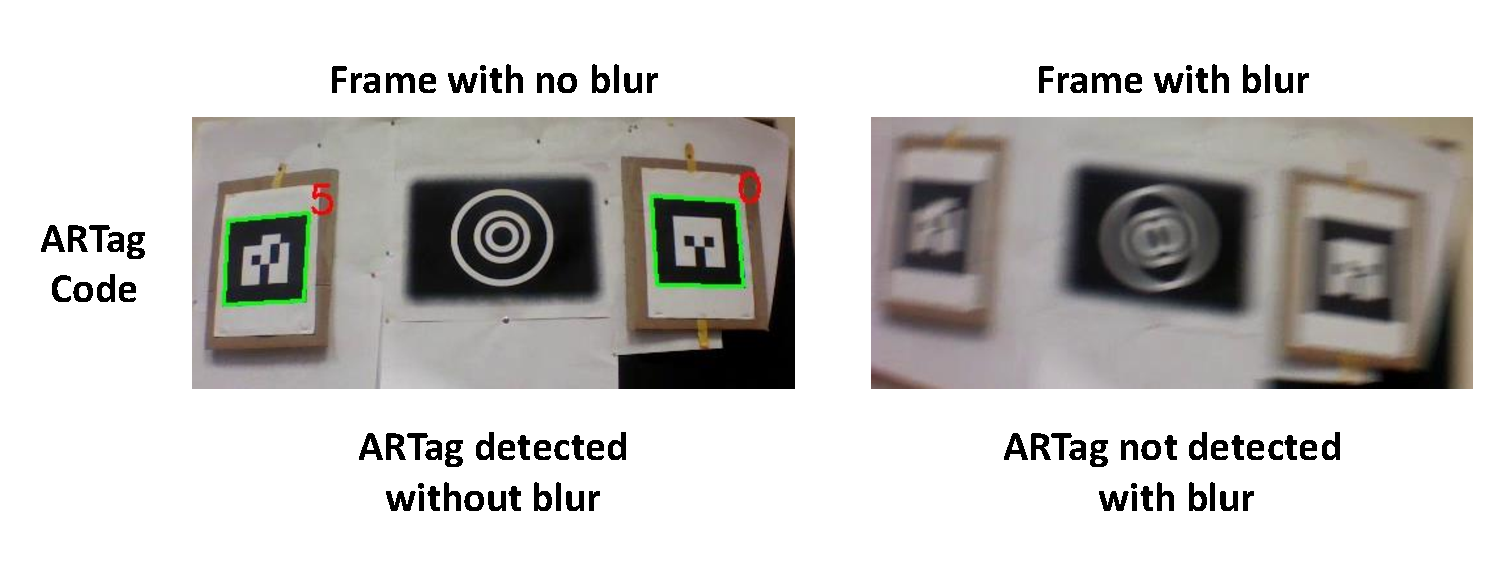
\includegraphics[width=0.98\linewidth]{figures/fiducial/ARTagBlur}
\caption[Problem of motion blur in ARTag]{Illustration of problem with ARTag.
There are two ARTags in the scene.
When there is no blur in the captured image(Left), both ARTags get detected
(indicated by green rectangle). But, when there is motion blur in the captured
image(Right), none of the ARTags get detected.}
\label{fig:ARTagBlur}
\end{figure}

\end{itemize}

\section{Our Contributions}
\begin{figure}[h!]
\centering
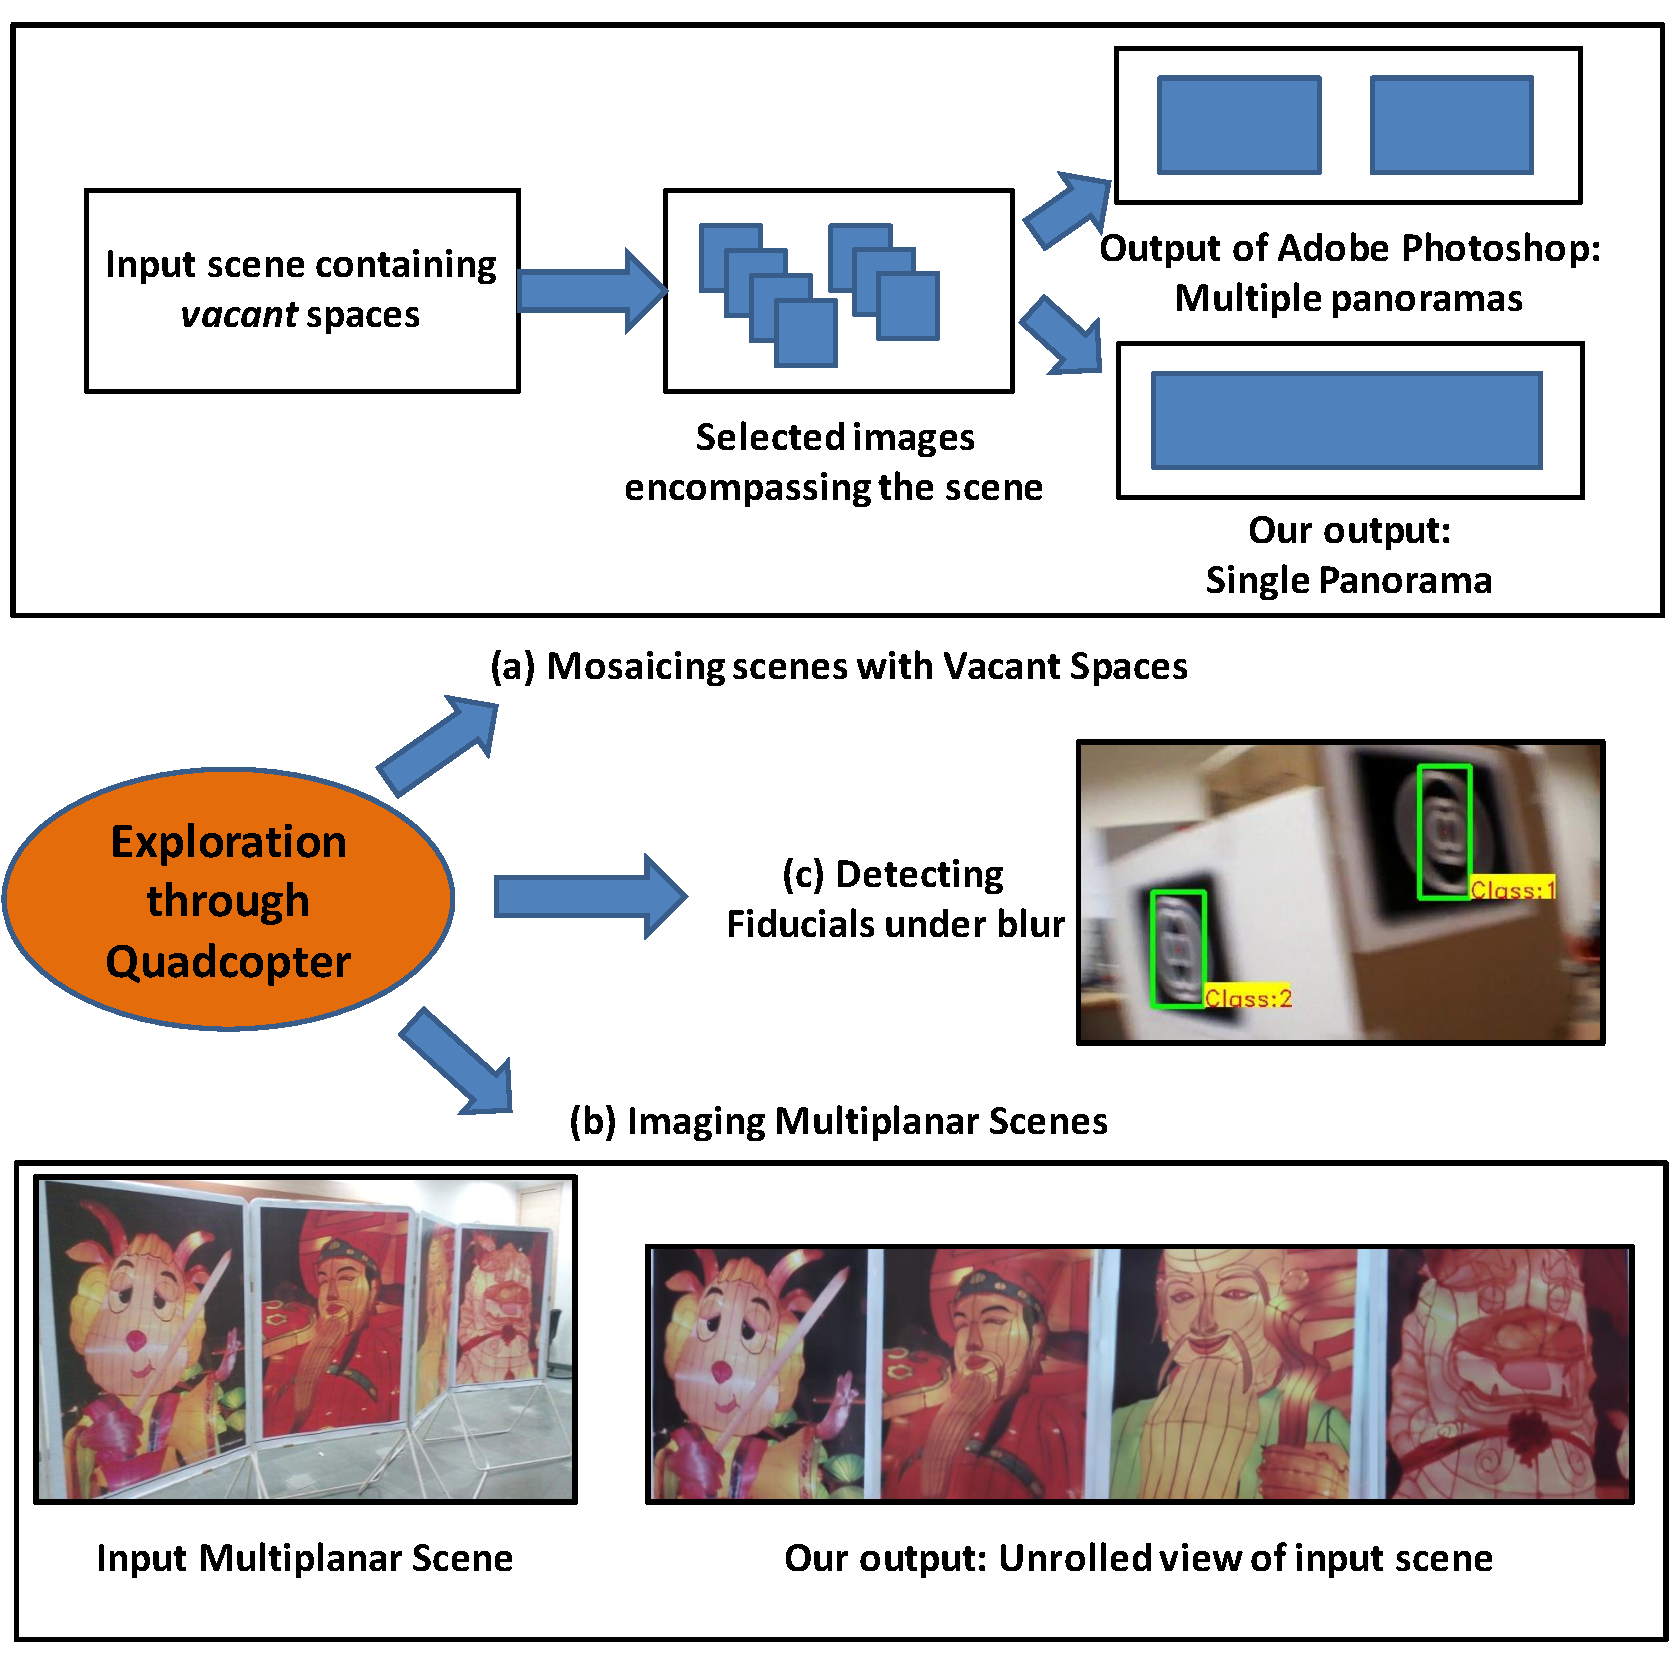
\includegraphics[width=0.98\linewidth]{figures/contributions2}
\caption[Our Contributions]{Our work involves techniques required for imaging
multiplanar surfaces through one or more quadcopters. (a) Shows mosaicing of a scene containing
vacant spaces. Two exhibits on a wall are separated by  a large vacant space
which makes homography based stitching methods ineffective. (b) Shows imaging
of a multiplanar scene through quadcopter. We imaged a multiplanar scene in such
a way that content on each plane is imaged with an orthographic view. Later we
combined a mosaic from each planar bounded region to get the  unrolled view of
an overall scene. (c) Shows our blur-resilient fiducials being detected in the
presence of motion blur, even from oblique angles.}
\label{fig:contributions}
\end{figure}

As shown in Fig. \ref{fig:contributions}, we develop an integrated solution to
explore scenes spread over single or multiplanar scenes through quadcopter. To
the best of our knowledge, we are the first to use quadcopter for:
\begin{itemize}
  \item Mosaicing scenes with vacant spaces  
  \item Imaging scenes spread over multiple planes autonomously   
\end{itemize}

Specific contributions made to achieve this goal and to address the above
mentioned challenges are:\\

\subsection{Mosaicing Scenes with Vacant Spaces}
\begin{figure}[h!]
	\centering
	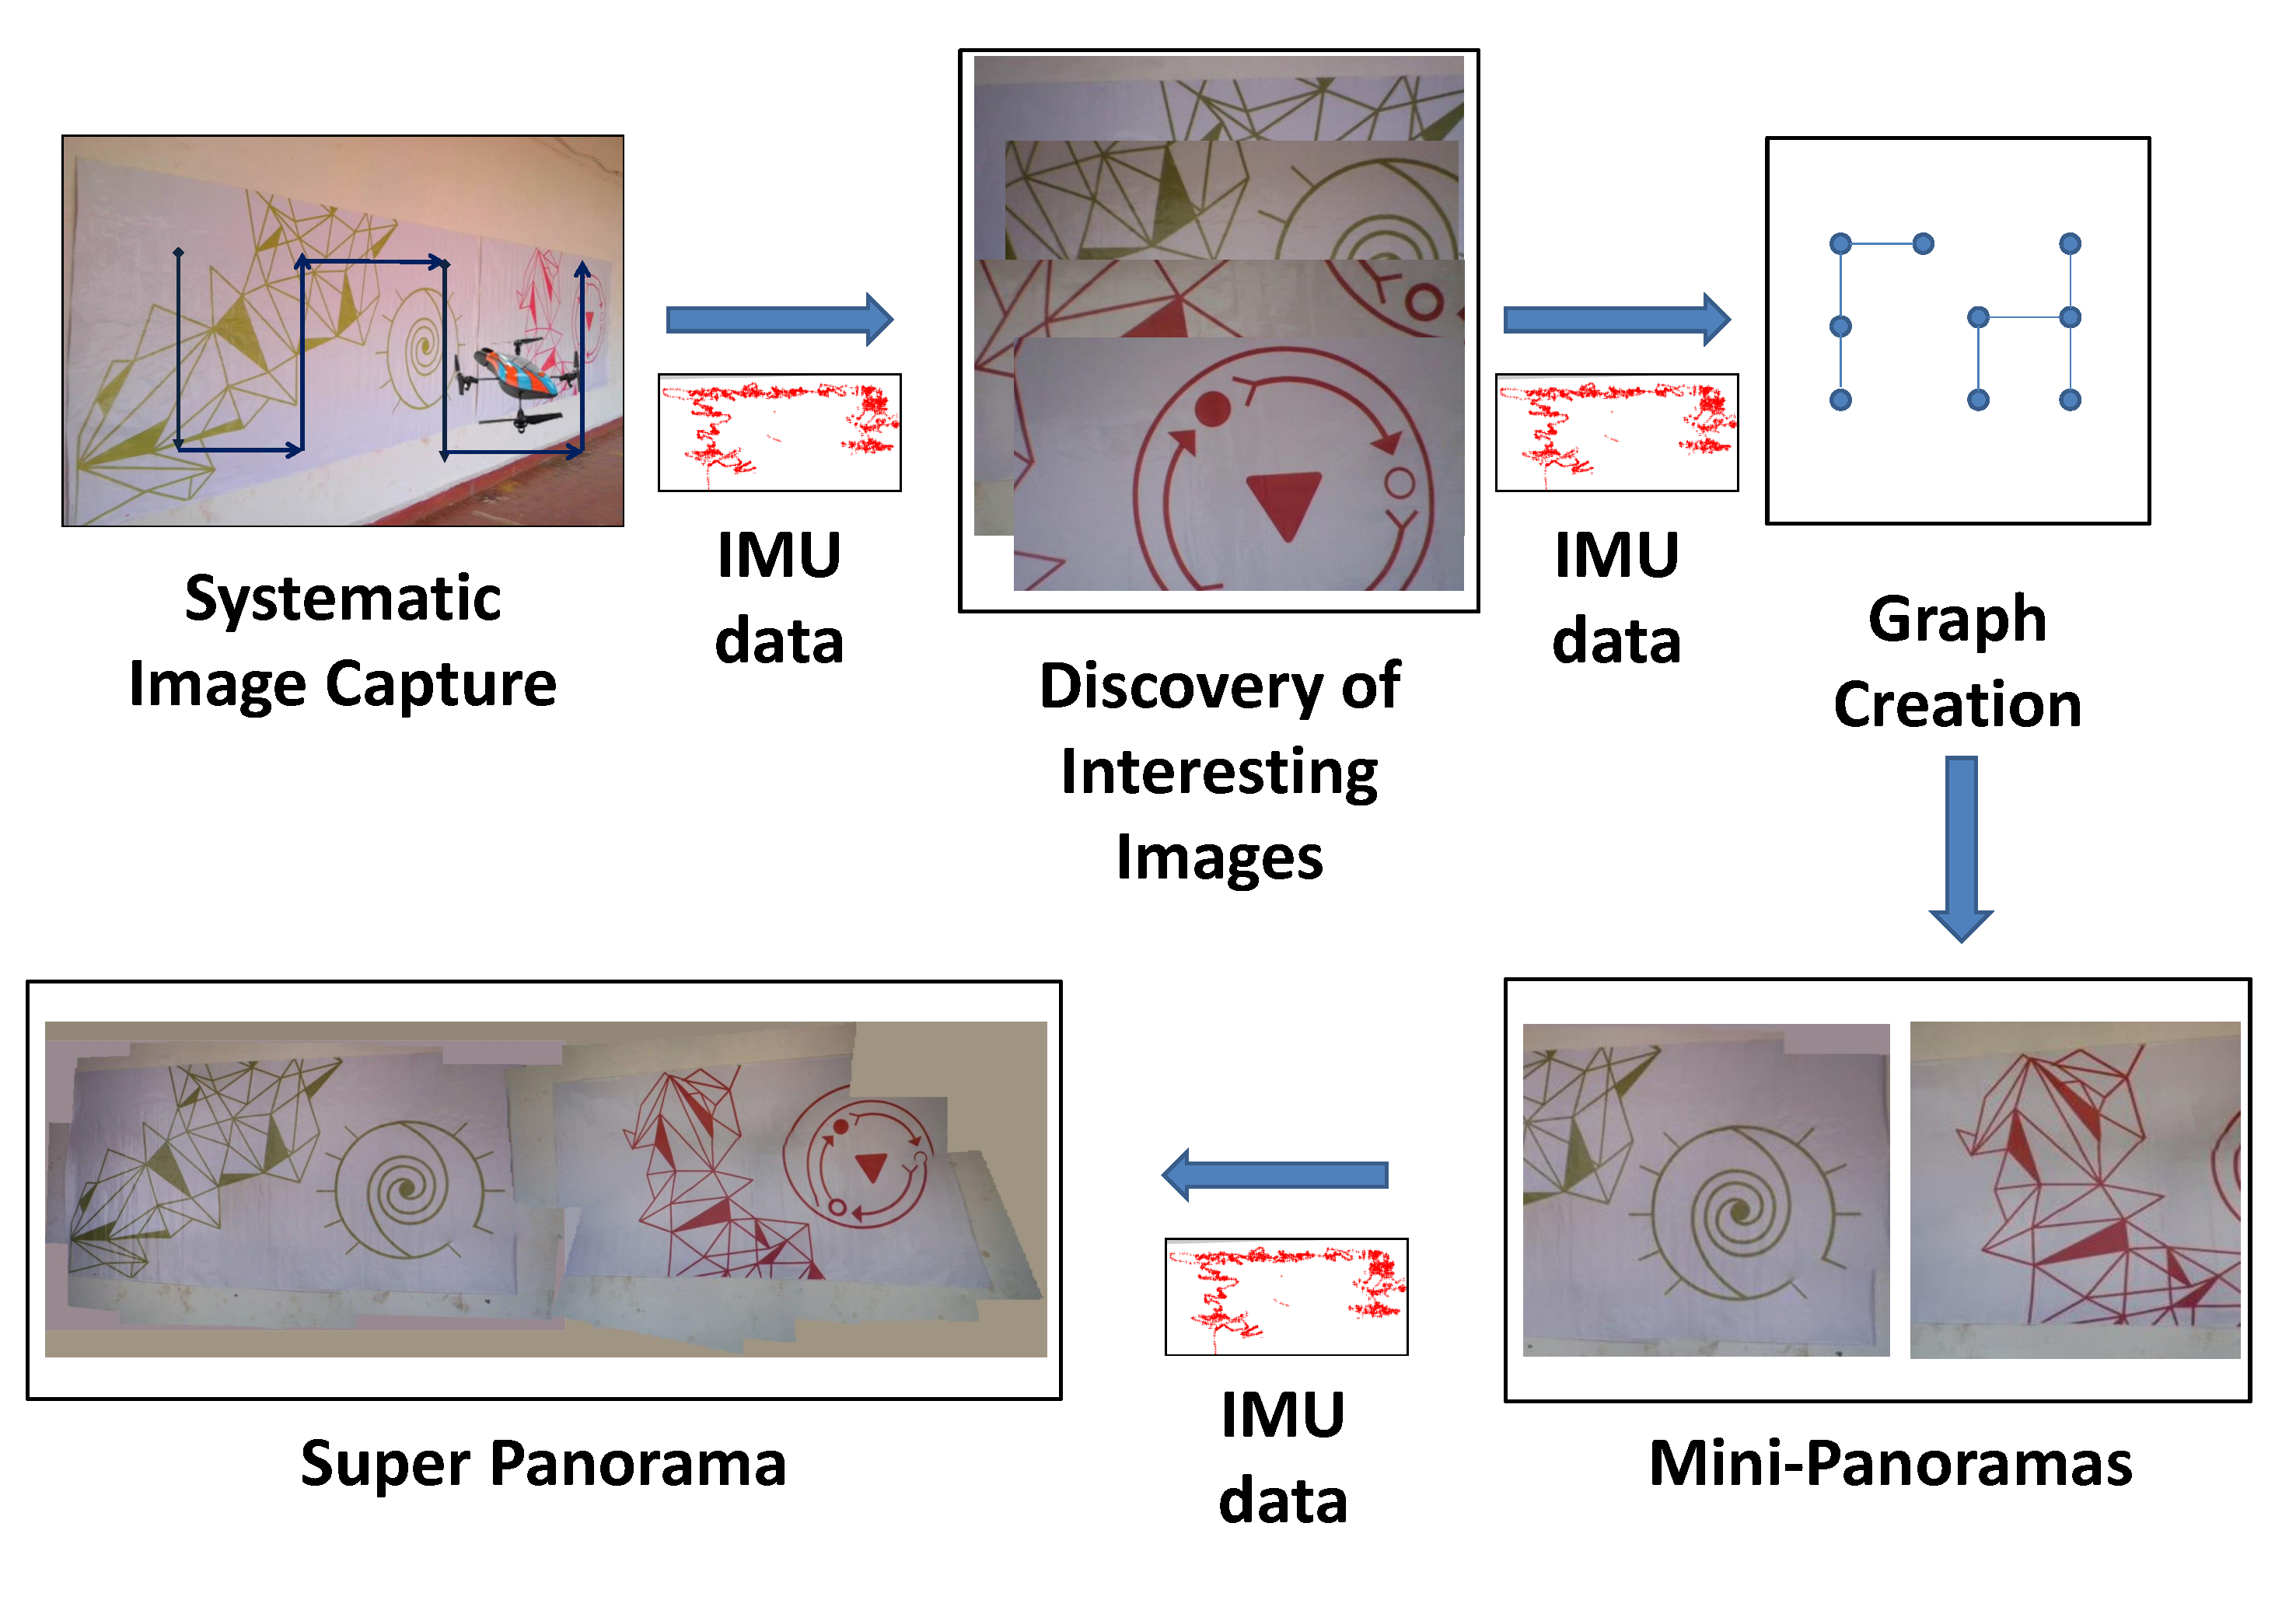
\includegraphics[width=0.98\linewidth]{figures/vacantSpaces/Workflow}
	\caption[Workflow]{ Overview of mosaicing scenes with vacant spaces: Input
	imagery is systematically acquired (top left) by a quadcopter.  In the next
    step, interesting images are found by clustering the video into
    regions based on positional data.  A graph is constructed using
    proximal images. For each connected component in a graph, standard
    stitching techniques are used to create mini-panoramas which are
    then joined together into a super panorama 
    again using IMU data.}
    \label{fig:vaccantSpaces_workflow} 
  \end{figure}
  
  We propose to solve the vacant space problem by using additional information
  available from an inexpensive quadcopter.  Quadcopter contains an inertial
measurement unit (IMU) that has positional information. We use the positional
information from IMU primarily for two purposes:
\begin{enumerate}
\item \textbf{Selection and ordering of images:}
We use the IMU data to select representative images from the video and arrange
them into rectangular grid according to the `spatial' neighborhood. It also
  disambiguates situations when multiple images that are spatially distant,
  have similar, repeated features.

\item \textbf{Super-panorama:} Whenever there are no features in
  the overlap region of two images, we use the IMU data to find the
  relative position of one mini-panorama with respect to another.
\end{enumerate}

However, IMU data on a quadcopter cannot be relied exclusively, or sometimes at
all, especially on inexpensive devices. Our experiments indicate that roll
and pitch angles (depending on the distances involved) may be completely off,
and so can the physical coordinates.  This is a consequence of jerky,
swift movements.  Complementing the IMU with information gleaned from
vision algorithms, however, may be a useful practice.

The method adopted is pictorially depicted in the overview shown in
Figure~\ref{fig:vaccantSpaces_workflow}.  In
brief, we systematically acquire a video of the scene, reduce the
input video to a manageable number of images, and finally combine the
images acquired from different positions into a mosaic. 

The result on a sample scene is shown in Figure~\ref{fig:vacantSpaces_result}.
In this experiment, the input stream had about 9000 input images.  Our selection algorithm
 pruned the video into $N=13$ images. A sample of the selected images are seen
 in Figure~\ref{fig:vacantSpaces_result}(a).  The scene as captured by a
 smartphone can also be seen, as well as the outputs of the state of the art
 stitchers, viz., AutoStitch\cite{autostitch} and Adobe
 PhotoShop\cite{photoshop}. Note that AutoStitch\cite{autostitch} is only able
 to stitch the upper half of the scene.  Our result
 Figure~\ref{fig:vacantSpaces_result}(e) clearly stands out in comparison.\\
  
  \begin{figure}[h!]
	\centering
	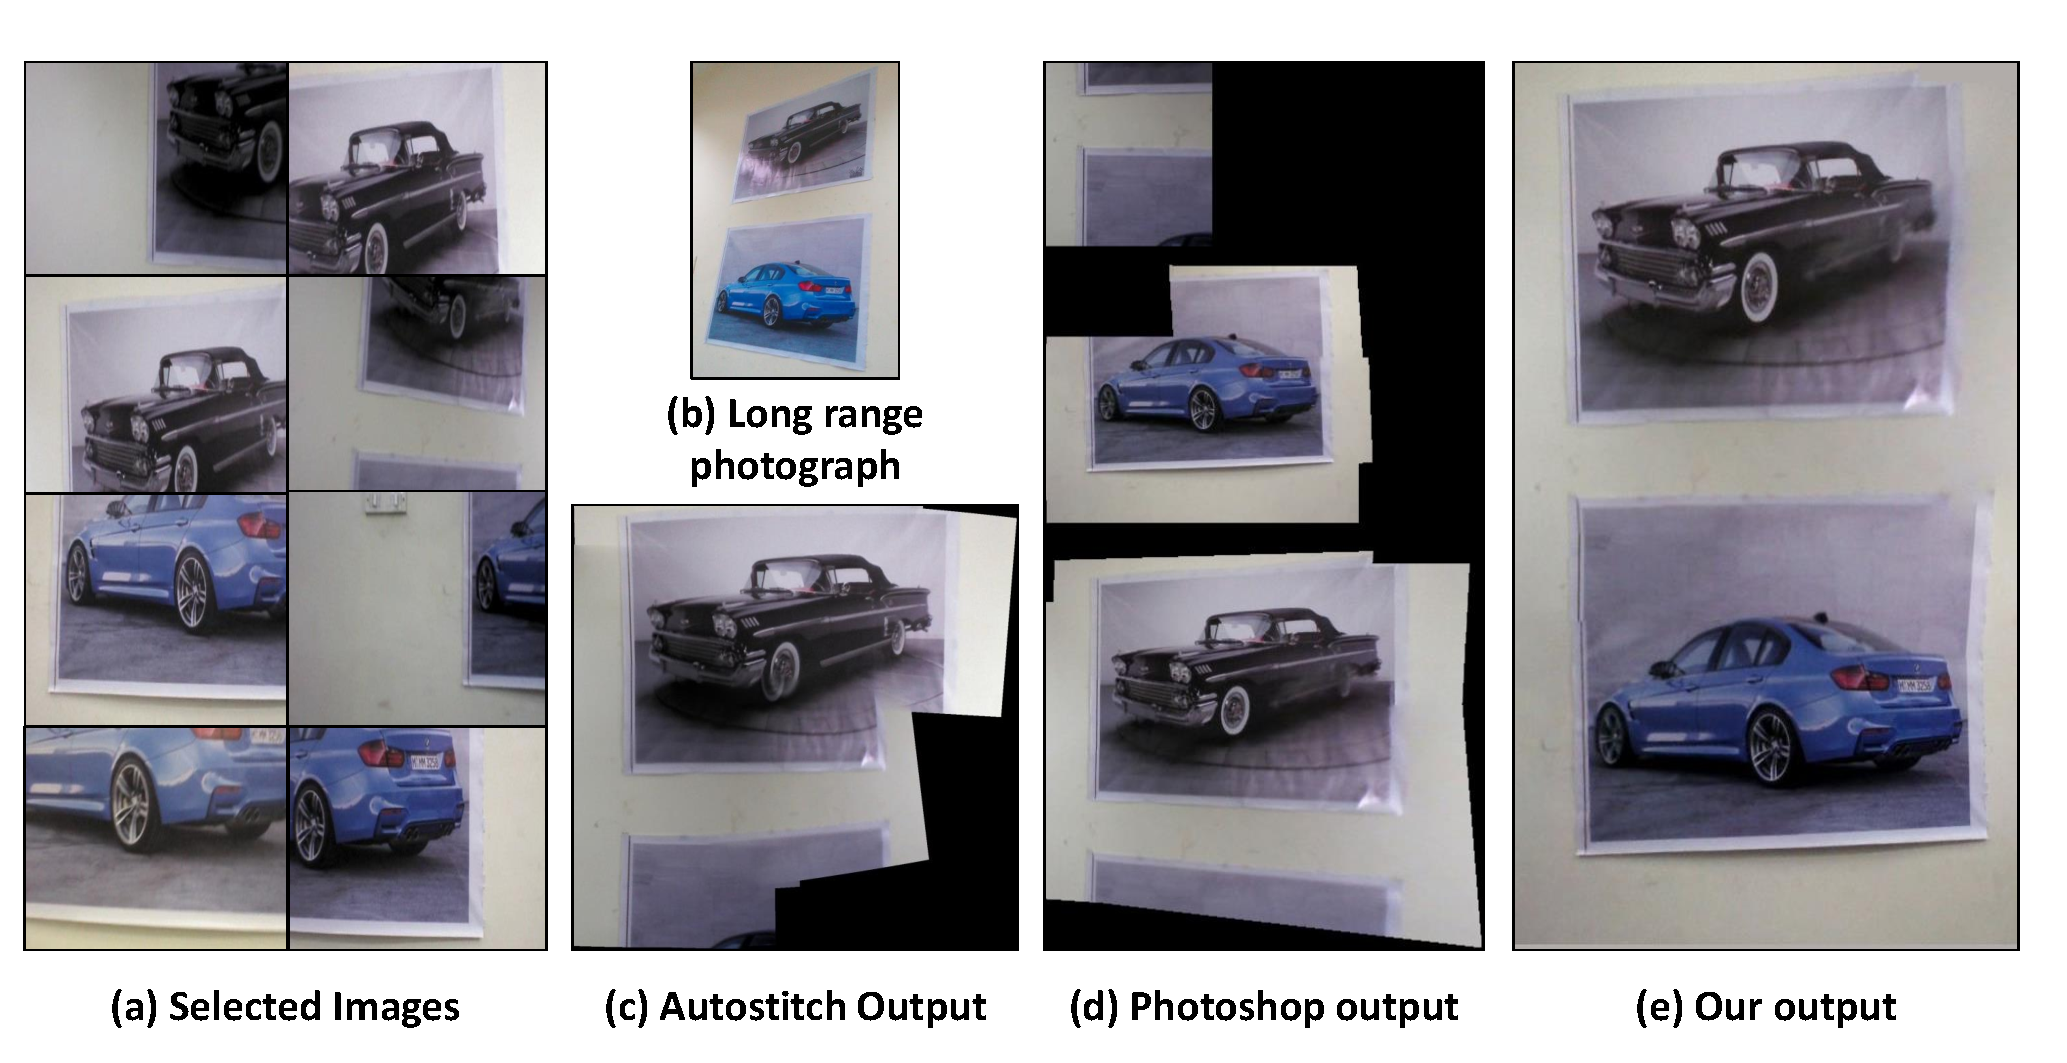
\includegraphics[width=0.98\linewidth]{figures/vacantSpaces/indoor_results}
	\caption[Result: Cars]{ (a) Pruned images from the quadcopter video using our
  saliency algorithm of (b) an indoor scene. This long range photograph
  has been captured separately by a smartphone camera only for the
  context. Notice a significant vacant space in the imagery.  (c)
  Output of AutoStitch -- only the upper half of the scene is output.
  (d) Output of Adobe Photoshop CS6 -- the vacant space posed a problem to the
  feature matching algorithm, so instead of a mosaic, individual
  pieces were output as mini-panoramas (e) Our output on the selected
  images. We are able to present the scene in high fidelity in an
  orthographic view.}	
	\label{fig:vacantSpaces_result}
	\end{figure}
  
\subsection{Autonomous Multiplanar Imaging through quadcopter}
\begin{figure}[h!]
\centering
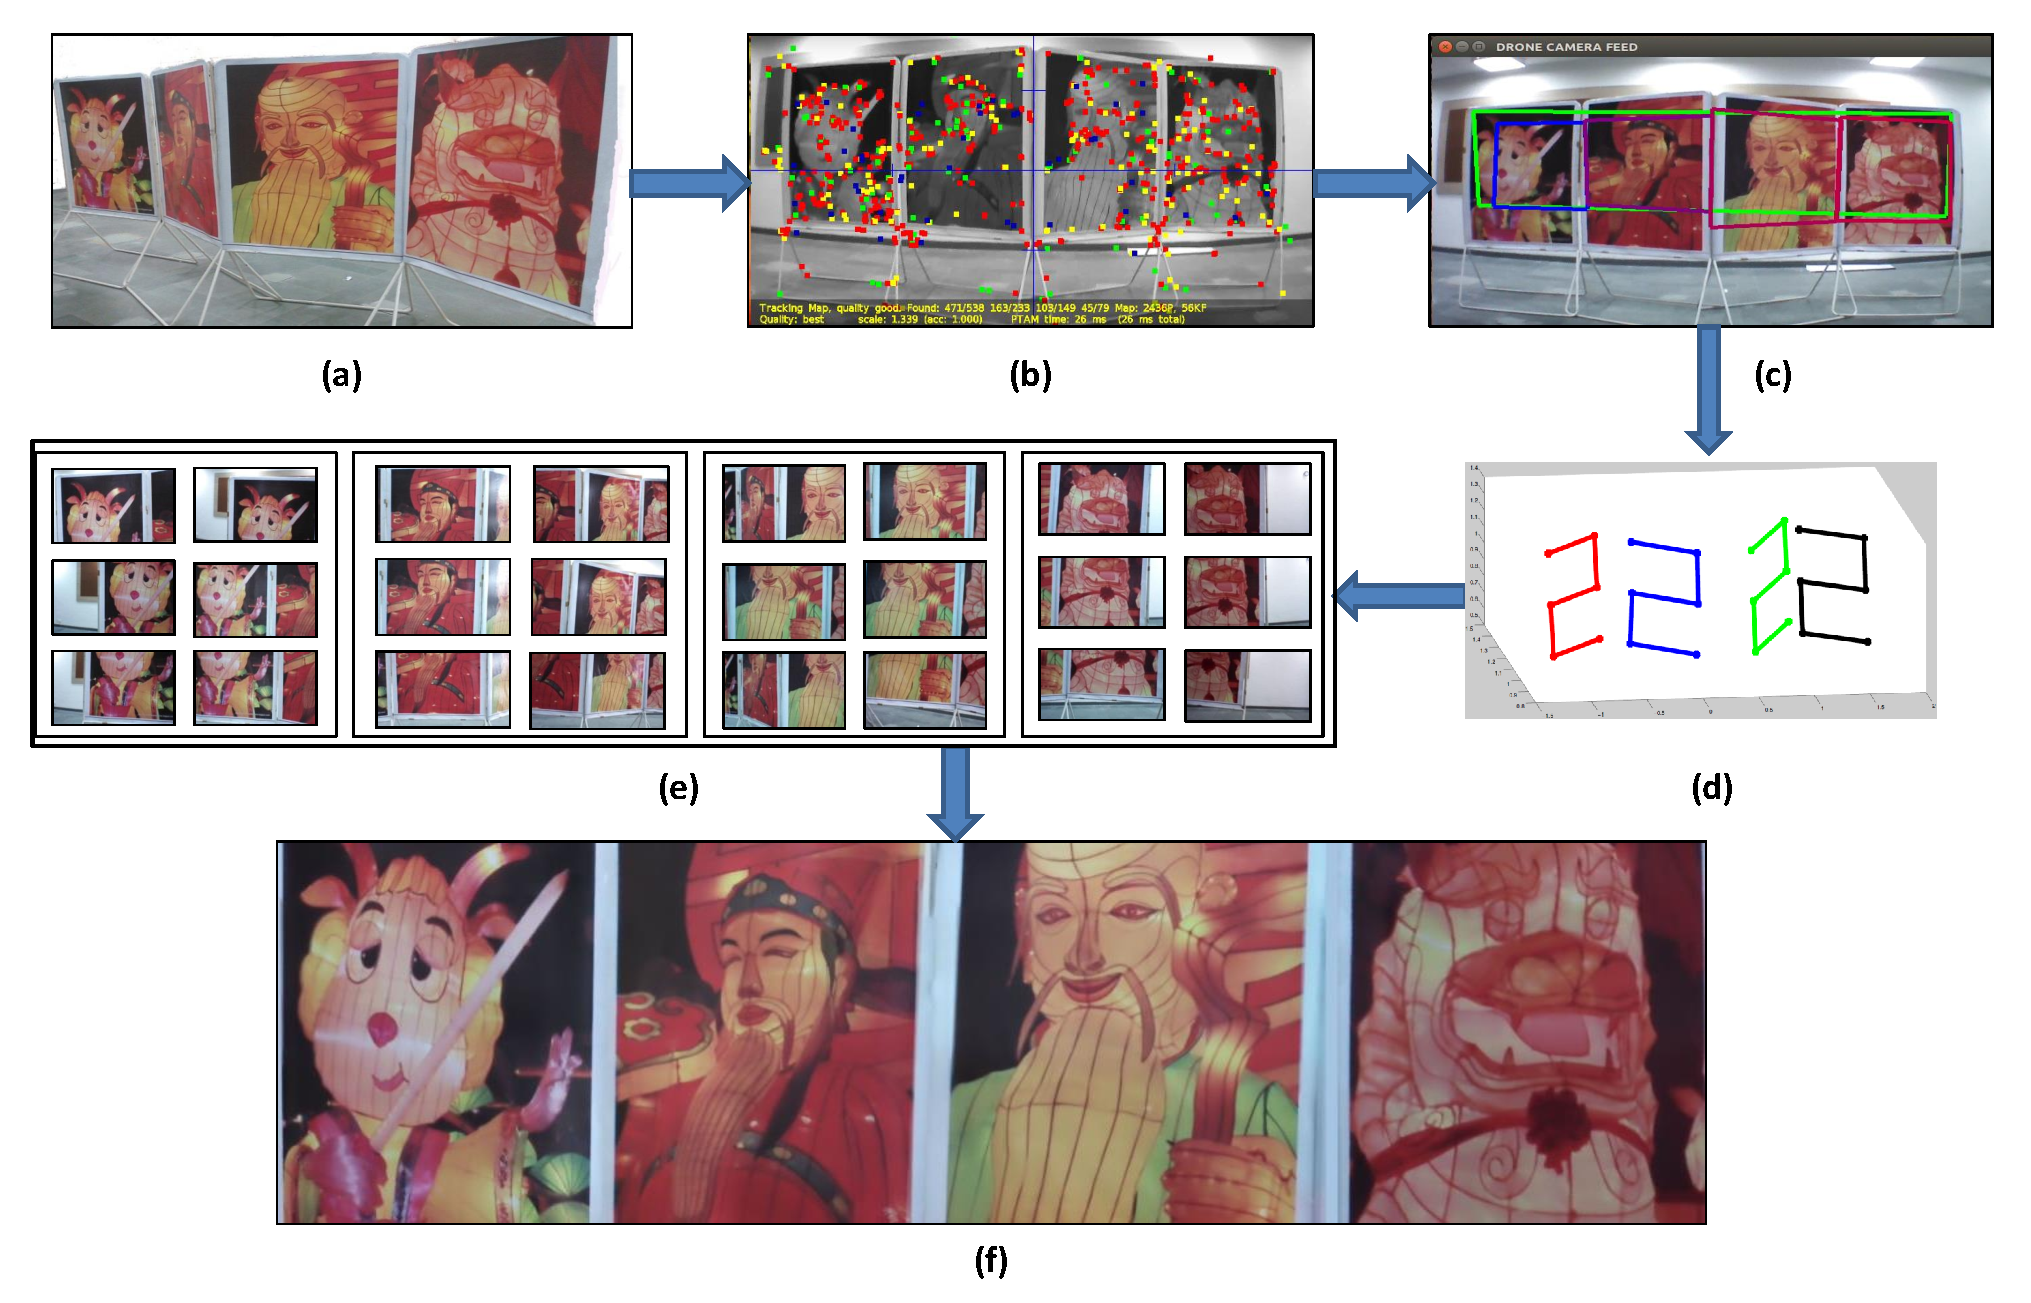
\includegraphics[width=0.98\linewidth]{figures/multiplanar/workflow}
\caption[Overflow of autonomous multiplanar imaging through quadcopter]{Overview
of Multiplanar Imaging through quadcopter:
(a) An input Scene to be imaged.
(b) Feature points in the scene are found and their 3D positions are estimated
using scale aware PTAM \cite{Engel12}. (c) Multiple planar bounded regions are
estimated using our algorithm. (d) For each bounded planar region, 3D camera
positions are calculated and overall path planning is done. (e) Videos are
captured at each target position. From each captured video, the appropriate
frame is found. (f) Individual mosaics are joined together to get final output.}
\label{fig:multiplanar_workflow}
\end{figure}

The mosaicing algorithms can mosaic only if the scene lies on a single planar
surface. But the real world is made of multiplanar as well as curved surfaces.
In fact, we have many circumstances where the input scene is spread over
multiple planes. In such cases, we would like to image each planar region
orthographically and then `unroll' the whole scene by joining the individual
mosaics so that we get the output mosaic of the input scene as if it is present
on a single plane.

The method adopted is pictorially depicted in the overview shown in Figure
\ref{fig:multiplanar_workflow}. In brief, we probe the
input scene through a quadcopter, calculate the 3D positions of feature points
using PTAM based method\cite{engel}. Later we use our algorithm, an improvement
over j-linkage\cite{jlinkage} to detect multiplanar bounded regions from the area
marked by the user through our user interface. Path planning is done for each
planar bounded region to find out the camera positions in such a way
that images captured from those positions encompass the scene in optimal manner.
The quadcopter is autonomously maneuvered along the estimated path and videos
are captured at target points. For each planar bounded region, the appropriate
frame from each video is found and then given to a mosaicing algorithm. 
Finally, all mosaics are joined together to get a full unrolled view.

Our experiments are done on various setups covering multiple planes.
In one such experiment, paintings were arranged in the convex
fashion as shown in Figure \ref{fig:multiplanar_result}(Top-Left). We have selected
the area to be imaged as shown in Figure \ref{fig:multiplanar_result}(Top-Right). In
the path planning stage, overall 30 (9 from the left plane, 12 from the middle
and 9 from the right plane) positions to cover full region are estimated.  Images
captured from those positions are mosaiced using our algorithm to get the final
mosaicing output as shown in the Figure \ref{fig:multiplanar_result}(Bottom).
\begin{figure}[h!]
	\centering
	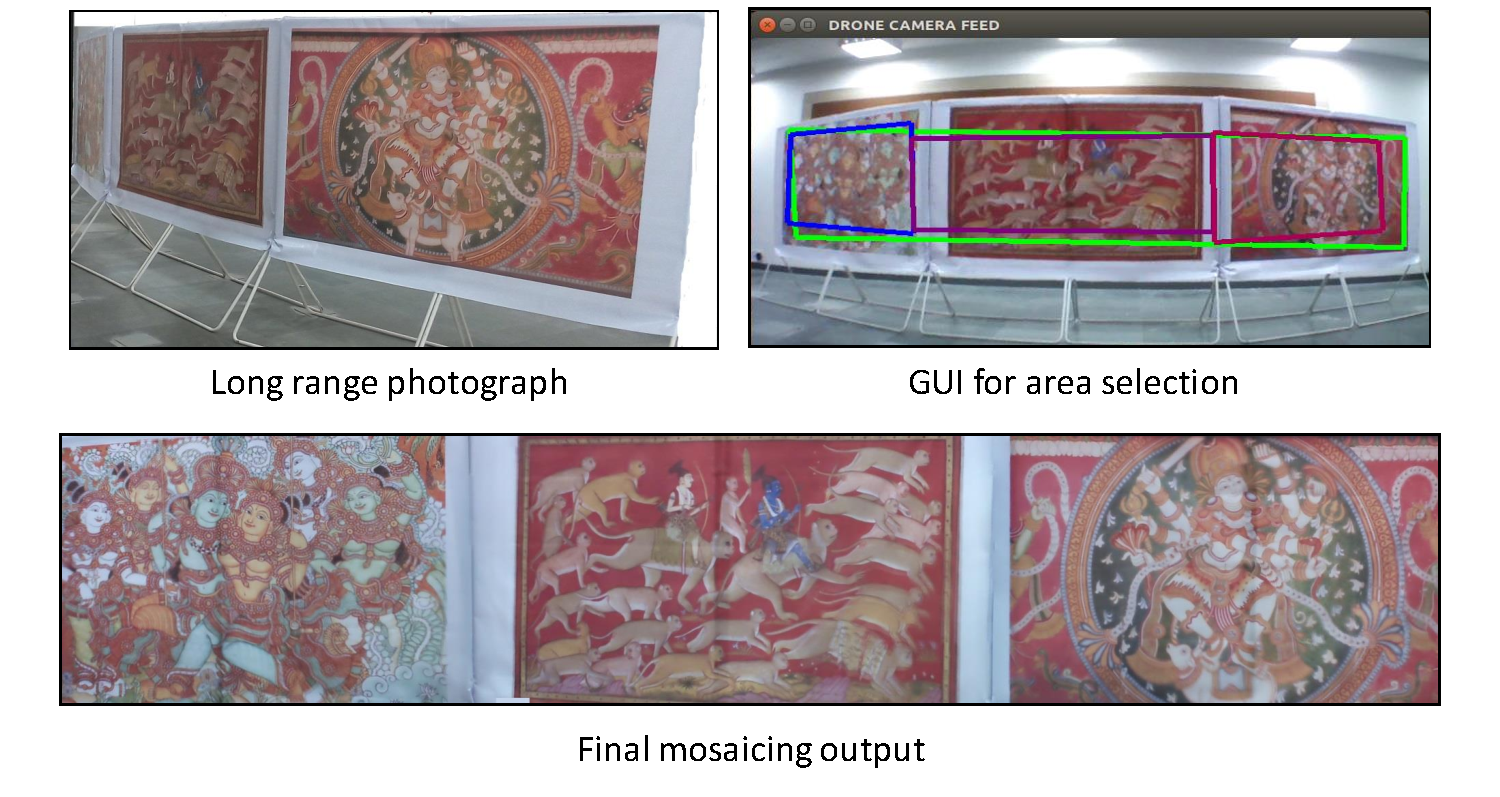
\includegraphics[width=0.98\linewidth]{figures/multiplanar/convexResult}
	\caption[Result: Imaging Convex Surface ]{There is an exhibition of Indian
	temple paintings arranged in convex fashion as shown in the long range photograph (top-left). Note that we
cannot cover all paintings with enough details simultaneously. We have selected
the area to be imaged as shown in GUI for area selection (top-right).
Green quadrilateral shows the user selected area while blue, violet and magenta
colored quadrilaterals represent the multiple planar bounded regions
estimated by our algorithm. In the path planning stage, overall 30 (9 from left
plane, 12 from middle and 9 from the right plane) positions were estimated to cover
the full region. Images captured from the estimated positions are mosaiced using
our algorithm to get the final mosaicing output as shown in the bottom image.}	
	\label{fig:multiplanar_result}
\end{figure}
	
\subsection{Blur Resilient Fiducials for Quadcopter}

\begin{figure}[h!]
\centering
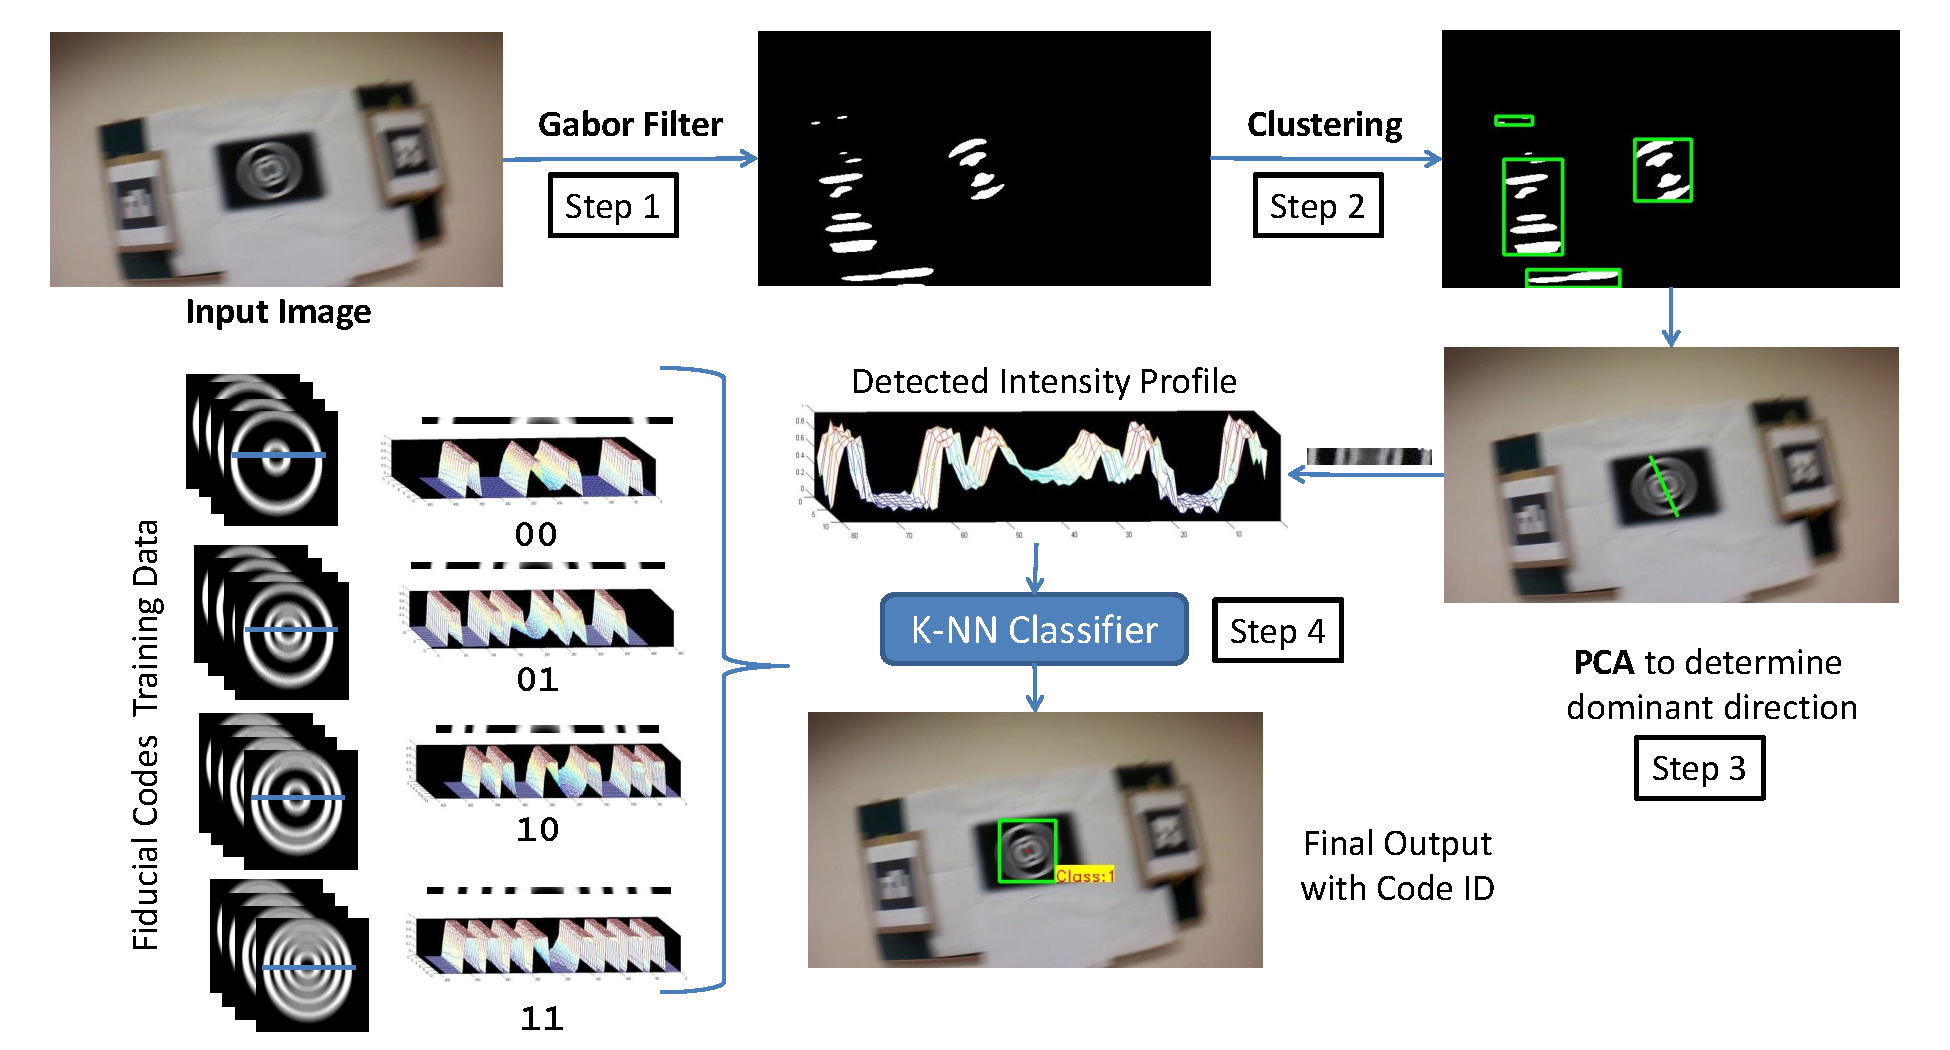
\includegraphics[width=0.98\linewidth]{figures/fiducial/overall_flow}
\caption[Overall Workflow of blur resilient fiducial detection algorithm]{An
overview of our fiducial detection algorithm.
    The four step process includes (Step 1) Filtering,
    (Step 2) Component clustering, (Step 3) Dominant direction determination
    and (Step 4) Classification using prior training data.}
 \label{fig:fiducial_workflow}
\end{figure}

Single quadcopter is not sufficient for imaging large multiplanar scenes due to
battery constraints. Instead, we may use multiple quadcopters in
collaboration for imaging multiplanar scenes. We have to identify each
quadcopter uniquely for accurate collaboration among multiple quadcopters. 

Generally, fiducial markers such as ARTag\cite{Fiala05} are used to identify
objects in environment. A problem with existing fiducials is that low-cost
quadcopters often exhibit very quick and erratic physical movements that result
in motion blur which is evident in the images captured from the quadcopter's
onboard camera. This motion blur has an adverse effect on the recognition of fiducial
markers. This can be seen in Figure \ref{fig:fiducials_result}(Top) where the
ARTag fiducial cannot be recognized due to motion blur. This is not too
surprising as most existing fiducials are not designed to handle motion blur.

Compounding this problem is the additional issue of dropped video
frames from the quadcopter's wireless communication module. This means
that not only is blur a problem, but there may be large
discontinuities in the pattern's position due to missing video
frames. This latter problem makes it challenging to apply tracking algorithms
that can exploit temporal coherence for determining the fiducial's position.

To address these problems, we propose a fiducial that is designed to be
resistant to motion blur. Our design is based on circles as shown in
Figure~\ref{fig:fiducials_result}(Bottom). The design is based on the
observation that motion blur from a quadcopter tends to be linear in nature. As
such, when our fiducial is blurred, there is no blur in the direction
perpendicular to the direction of motion. This allows the signature of the
fiducial to remain intact in any direction.

Figure~\ref{fig:fiducial_workflow} shows the process involved in fiducial
detection. Our detection algorithm has four steps. In Step~1, we apply a Gabor
filter on the image to isolate the potential locations of the pattern.  In
Step~2, we find clusters of patches in the Gabor output.  In Step~3, we perform
the Principal Component Analysis (PCA) on each cluster to find the dominant
direction unaffected by the blur.  Finally in Step~4, based on the
direction detected, we extract the intensity profile of the pattern
and classify the fiducial.

\begin{figure}
\begin{subfigure}[b]{0.24\textwidth}
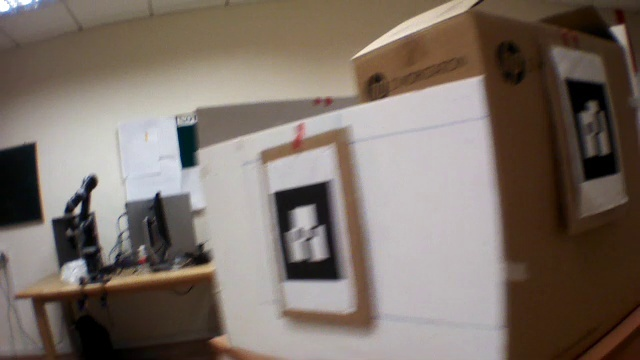
\includegraphics[width=\linewidth]{figures/fiducial/setup_artag/output_79.jpg}
\end{subfigure}
\begin{subfigure}[b]{0.24\textwidth}
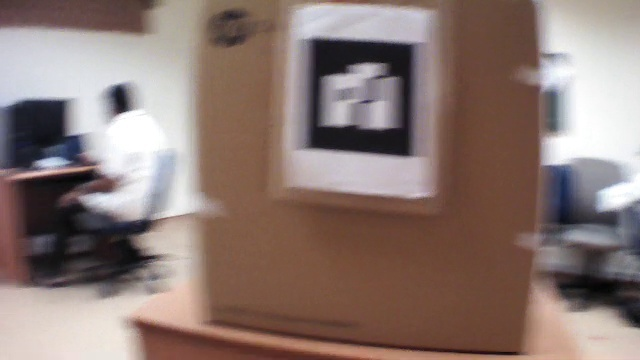
\includegraphics[width=\linewidth]{figures/fiducial/setup_artag/output_150.jpg}
\end{subfigure}
\begin{subfigure}[b]{0.24\textwidth}
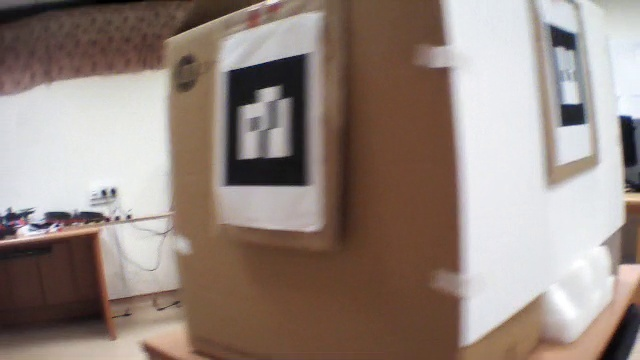
\includegraphics[width=\linewidth]{figures/fiducial/setup_artag/output_194.jpg}
\end{subfigure}
\begin{subfigure}[b]{0.24\textwidth}
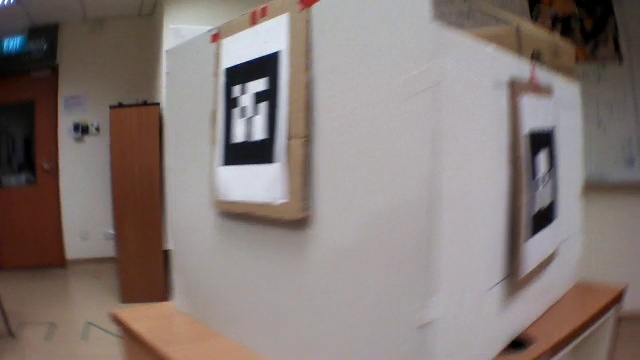
\includegraphics[width=\linewidth]{figures/fiducial/setup_artag/output_480.jpg}
\end{subfigure}\\
\begin{subfigure}[b]{0.24\textwidth}
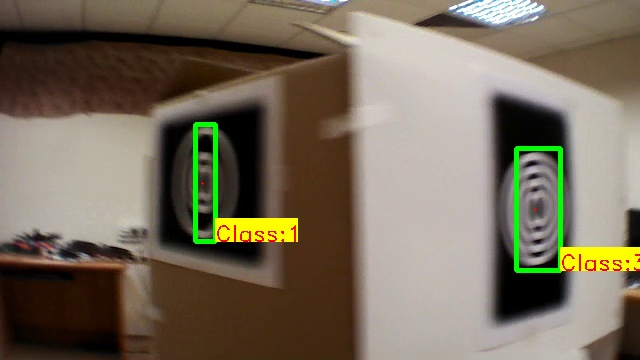
\includegraphics[width=\linewidth]{figures/fiducial/setup_our/output_6/output_514.jpg}
\end{subfigure}
\begin{subfigure}[b]{0.24\textwidth}
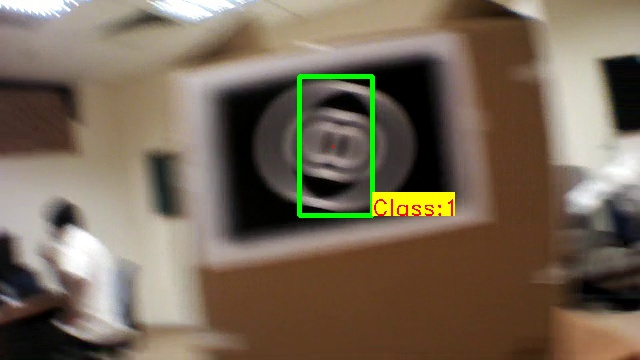
\includegraphics[width=\linewidth]{figures/fiducial/setup_our/output_2/output_64.jpg}
\end{subfigure}
\begin{subfigure}[b]{0.24\textwidth}
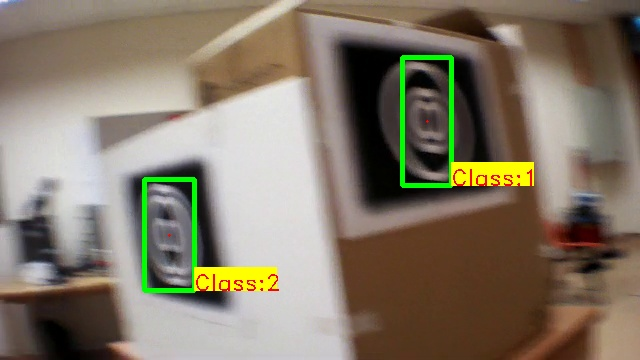
\includegraphics[width=\linewidth]{figures/fiducial/setup_our/output_2/output_35.jpg}
\end{subfigure}
\begin{subfigure}[b]{0.24\textwidth}
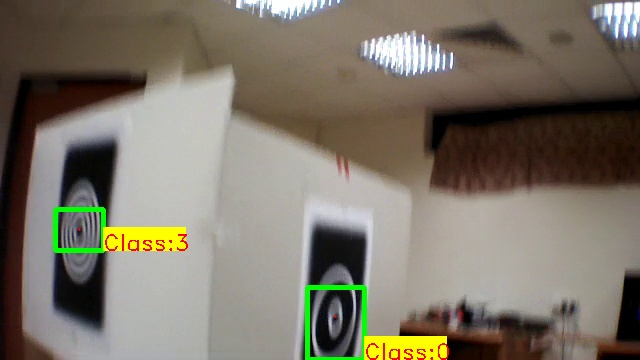
\includegraphics[width=\linewidth]{figures/fiducial/setup_our/output_6/output_943.jpg}
\end{subfigure}
\caption[Comparison of ARTag and our fiducial when quadcopter is
  revolving around our setup]{Comparison of ARTag and our fiducial when quadcopter is
  revolving around our setup. 
\textbf{Top} ARTags are not detected, shown by an absence of green rectangles.
\textbf{Bottom} In similar conditions, proposed fiducials are successfully
detected. The overall detection rate of proposed fiducials is 90\% while that of
ARTags is around 60\%. }
\label{fig:fiducials_result}
\end{figure}
	
\section{Organization of the thesis}
The remainder of the thesis is organizes as follows:\\

\noindent \textbf{Chapter 2} explains the details of a quadcopter focussing on
control and navigation aspects. Here, we also present previously published work
in the area of mosaicing, autonomous navigation of quadcopter as well as
fiducials. We use this chapter as an opportunity to establish and contrast the
scope of this thesis with respect to prior art.\\

\noindent \textbf{Chapter 3} elaborates our proposed method for ``Mosaicing
Scenes with Vacant Spaces'' using quadcopter. Proposed method fuses positional information
from quadcopter with images to first, find out the position from which each
image is taken and accordingly sort the images in two dimensional grid; second,
use positional information to join two adjacent images which have very few features
in common (and hence cannot be stitched using the homography-based method).\\

\noindent \textbf{Chapter 4} provides an overview of our approach
for imaging multiplanar scenes though quadcopter. Issues such as detection of
multiplanar bounded regions and path planning for efficient imaging of multiplanar scenes
are addressed.\\

\noindent \textbf{Chapter 5} elaborates on our design of blur
resilient fiducial for identification of objects under a heavy motion blur. We
have also proposed algorithm for robust detection of our blur resilient
fiducial in this chapter.\\
 
 \noindent \textbf{Chapter 6} concludes the thesis by summarizing our
 contributions.
  We have also discussed possible ways to extend some of the ideas proposed in this thesis.